
%(BEGIN_QUESTION)
% Copyright 2006, Tony R. Kuphaldt, released under the Creative Commons Attribution License (v 1.0)
% This means you may do almost anything with this work of mine, so long as you give me proper credit

{\it RTDs} are often used inside of bridge circuits to convert a temperature measurement into a voltage:

$$\includegraphics[width=15.5cm]{i00040x01.eps}$$

Assume that the bridge is balanced when the RTD is at its lower range value (LRV).  Identify:

\begin{itemize}
\item{} The polarity of the voltage across all bridge resistors.
\item{} The polarity of the voltage sensed by the measuring instrument as temperature increases toward the URV.
\item{} Which variable resistance ($R_1$ or $R_3$) adjusts {\it zero}.
\item{} Which variable resistance ($R_1$ or $R_3$) adjusts {\it span}.
\item{} One electrical fault (open or short) resulting in a positive over-range ($>$ 100 \% temp.) reading.
\item{} One electrical fault (open or short) resulting in a negative over-range ($<$ 0 \% temp.) reading.
\end{itemize}

Also, explain {\it why} you have identified the zero and span adjustment resistors as such:

\vfil 

\underbar{file i00040}
\eject
%(END_QUESTION)





%(BEGIN_ANSWER)

This is a graded question -- no answers or hints given!

%(END_ANSWER)





%(BEGIN_NOTES)


%INDEX% Measurement, temperature: RTD (bridge circuit)

%(END_NOTES)


